\subsubsection{The Kaus (2010) Brick}
\label{sec:benchmarks-the-kaus_2010-brick}

\textit{This section was contributed by John Naliboff, Marcel Saaro and Cedric Thieulot.}

This setup is borrowed from Kaus (2010) \cite{kaus10}. The domain is a Cartesian box of size $(L_x\times L_y)=(40~\si{\km}\times10~\si{\km})$.
The setup is shown in Fig.~\ref{fig:kaus_brick}. 
The viscous inclusion of size $(800~\si{\meter} \times 400\si{\meter})$ is centered at the bottom of the domain. Its viscosity is $\eta_i=10^{20}~\si{\pascal\second}$.

The brick material is characterised by an (elasto-)visco-plastic
rheology following a Drucker-Prager yield criterion with a cohesion $c=40~\si{\mega\pascal}$ and angle of 
friction $\phi=30\si{\degree}$. The elastic shear modulus is set to $G=50\cdot10^{10}~\si{\pascal}$.

Both materials have a density of $\rho=2700~\si{\kg\per\cubic\meter}$. The gravity is pointing downwards with $g=10~\si{\meter\per\square\second}$.
The flow is assumed to be isothermal and incompressible.

The boundary conditions are free slip at the bottom and sides and stress free at the top (free surface). The horizontal component of the velocity is prescribed on the sides such that it results in a background strainrate of $\dot{\varepsilon}=2\cdot 10^{-15}~\si{\per\second}$. By reversing the values on both boundaries the brick can be put in compression or extension. 

The background resolution is composed of $100\times25$ repetitions, i.e. a resolution of $400~\si{\m}$. The model runs for $20~\si{\kilo\year}$.

\begin{figure}[h]
\centering
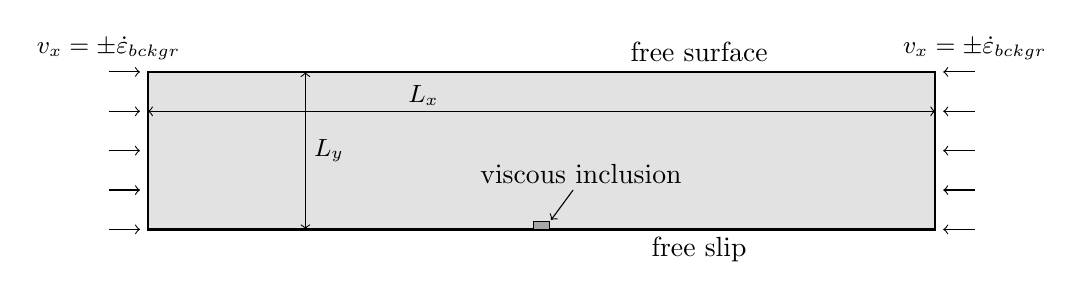
\begin{tikzpicture}
  \draw[fill=gray!23,gray!23](0,0) rectangle (10,2);
  %\draw[step=0.5cm,gray,very thin] (0,0) grid (10,8); %background grid
  
  % left part of drawing
  
  %domain
  \draw[fill=gray!23,thick](0,0) rectangle (10,2);
  %seed
  \draw[fill=gray!70](4.9,0) rectangle (5.1,0.1);
  %left arrows
  \draw [->] (-0.5,0) -- (-0.1,0);
  \draw [->] (-0.5,0.5) -- (-0.1,0.5);
  \draw [->] (-0.5,1) -- (-0.1,1);
  \draw [->] (-0.5,1.5) -- (-0.1,1.5);
  \draw [->] (-0.5,2) -- (-0.1,2);
  %right arrows
  \draw [<-] (10.1,0) -- (10.5,0);
  \draw [<-] (10.1,0.5) -- (10.5,0.5);
  \draw [<-] (10.1,1) -- (10.5,1);
  \draw [<-] (10.1,1.5) -- (10.5,1.5);
  \draw [<-] (10.1,2) -- (10.5,2);
  
  \node[] at (7,-0.25) {free slip};
  \node[] at (7,2.25) {free surface};
  
  \node[] at (-0.5,2.3) {\small $v_x=\pm \dot{\varepsilon}_{bckgr}$};
  \node[] at (10.5,2.3) {\small $v_x=\pm \dot{\varepsilon}_{bckgr}$};
  
  \draw [<-] (5.12,0.12) -- (5.4,0.5);
  \node[] at (5.5,0.7) {viscous inclusion};
  
  \draw [<->,thin] (0,1.5) -- (10,1.5);
  \node[] at (3.5,1.7) {\small $L_x$};
  
  \draw [<->,thin] (2,0) -- (2,2);
  \node[] at (2.3,1) {\small $L_y$};
  
  \end{tikzpicture}
\caption{\it Setup for the Kaus (2010) brick.}
\label{fig:kaus_brick}
\end{figure}

There is a python script included to generate Fig.-\ref{fig:kaus_brick_result}. The script is based on the one for plotting the strain rate field for the visco-elasto-plastic block.

\begin{figure}[h]
\centering
\includegraphics[width=12cm]{kaus10_vep.pdf}
\caption{The evolution of the shear bands over time shown by plotting the second strain rate invariant.}
\label{fig:kaus_brick_result}
\end{figure}